\begin{alist}
\item Επειδή $\sigma\upsilon\nu\omega = -\dfrac{1}{2}$ και $\eta\mu\omega > 0$, η γωνία θα βρίσκεται στο $2^0$ τεταρτημόριο του τριγωνομετρικού κύκλου. \\
Το μέτρο της γωνίας είναι $\omega = \dfrac{2\pi}{3}$ διότι $\sigma\upsilon\nu\omega = -\dfrac{1}{2} \Leftrightarrow \sigma\upsilon\nu\omega = -\sigma\upsilon\nu\left(\dfrac{\pi}{3}\right) = \sigma\upsilon\nu\left(\pi - \dfrac{\pi}{3}\right) = \sigma\upsilon\nu\dfrac{2\pi}{3}$.

\item Για τη τριγωνομετρική εξίσωση για $\varphi \in \mathbb{R}$ έχουμε:
\[\sigma\upsilon\nu\varphi = -\frac{1}{2} \Leftrightarrow \sigma\upsilon\nu\varphi = -\sigma\upsilon\nu\frac{\pi}{3} = \sigma\upsilon\nu\left(\pi - \frac{\pi}{3}\right) = \sigma\upsilon\nu\frac{2\pi}{3} \Leftrightarrow \sigma\upsilon\nu\varphi = \sigma\upsilon\nu\frac{2\pi}{3}\]
τότε $\varphi = 2\kappa\pi + \dfrac{2\pi}{3}$ ή $\varphi = 2\kappa\pi - \dfrac{2\pi}{3}$ με $\kappa \in \mathbb{Z}$.
\end{alist}
\begin{center}
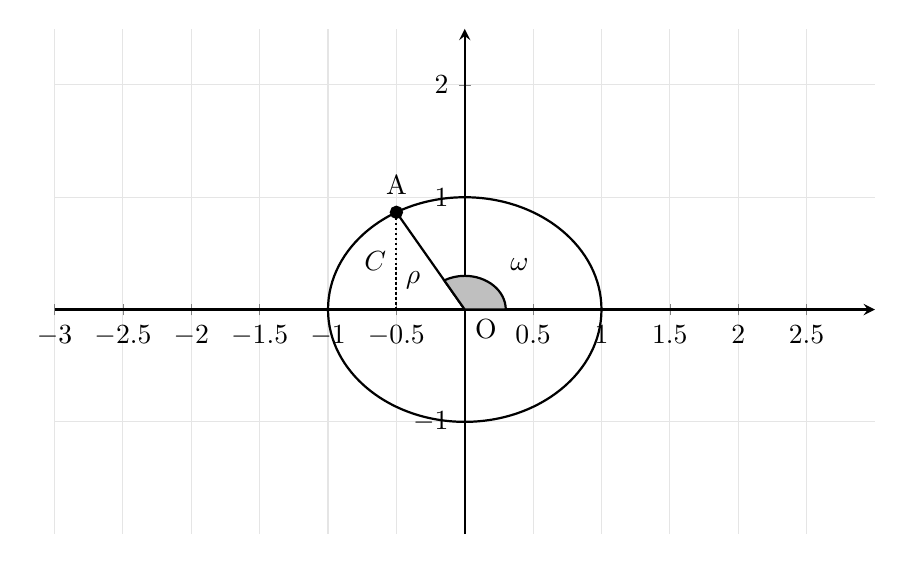
\begin{tikzpicture}
\begin{axis}[
    axis lines=middle,
    xmin=-3, xmax=3,
    ymin=-2, ymax=2.5,
    xtick={-3,-2.5,-2,-1.5,-1,-0.5,0,0.5,1,1.5,2,2.5},
    ytick={-1,1,2},
    grid=both,
    grid style={solid, gray!20},
    thick,
    width=12cm, height=8cm,
    samples=100
]
\draw[black, thick] (0,0) circle [radius=1];
\addplot[mark=*, fill=black] coordinates {(-0.5, 0.866)} node[above, yshift=1mm] {A};
\draw[thick] (0,0) -- (-0.5, 0.866) node[midway, below left] {$\rho$};
\draw[densely dotted, thick] (-0.5, 0) -- (-0.5, 0.866) node[midway, left] {$C$};
\draw[fill=gray!50] (0,0) -- (0.3,0) arc[start angle=0, end angle=120, radius=0.3] -- cycle;
\node at (0.4, 0.4) {$\omega$};
\node[below right] at (0,0) {O};
\end{axis}
\end{tikzpicture}
\end{center}
